\chapter{Quadcopter Test}
\label{chap5}

\section{Introduction}

The main objective of this research project is to determine the pose estimation accuracy of an airborne quadcopter in the outdoors. This can be done by comparing a quadcopter's on-board pose estimate with the pose measurement of an external measurement device.  

In Chapter~\ref{chap3}, a computer vision pose measurement system (CVS) was designed and tested and its pose measurement error was determined. It was found that the measurement data produced by the CVS is complex, high dimensional and interdimensionally dependant, as shown by the covariance matrix of Equation~\ref{eq:covariance-matrix}. This makes it hard to estimate the measurement error for any given pose measurement vector produced by the CVS.\@ 

Neural networks excel at detecting underlying relationships within data if they are properly designed and trained. In Chapter~\ref{chap4} a radial basis function neural network (RBFNN) was trained to be able to do this, since they have been proven to work well with complex, noisy and non-linear data. The accuracy of the trained RBFNN was verified by an additional data set and is ready to be used in a flight test with a quadcopter. 

The trained RBFNN was used with data gathered from a test flight from a quadcopter. This chapter sets out to discuss the design and details of the flight tests that were conducted, including the testing procedure, conditions and data processing. Then the results are presented and discussed, followed by a brief discussion on the data and results gathered thus far. 

\section{Flight Test Design and Procedure}

Work was done to ensure that the flight tests were performed where it would produce meaningful results without posing a safety risk to surrounding bystanders and equipment. This section discusses the planning that went into the flight test,, as well as the equipment that was used. It also describes the test location and procedure, as well as the data processing involved.  

\subsection{Flight Test Design}

This subsection describes the flight test design, including the equipment, the location and testing conditions.

\subsubsection{Equipment}

The equipment and facilities that were required and used for the flight tests are given as follows:

\begin{itemize}
    \item CVS camera and laptop.
    \item Suncopter quadcopter.
    \item Certified unmanned aerial vehicle pilot.
    \item Calibration board.
    \item Isolated test site. 
\end{itemize}

The details of the CVS are discussed in Chapter~\ref{chap3}. It consists of a camera, which captures the image data, and a laptop which records and processes the data. A certified unmanned aerial vehicle (UAV) pilot was used for safety reasons since the quadcopter will be flown in close proximity to people and other equipment. The calibration board is used in conjunction with the CVS to provide the pose data of the quadcopter. Here, the calibration board is an ISO A3-sized\footnote{Paper size of $\SI{297}{\mm}\times\SI{432}{\mm}$}, $6\times5$ square chessboard pattern calibration board. 

The Suncopter quadcopter is a custom-built quadcopter for the Solar Thermal Energy Research Group's (STERG) research purposes. The Suncopter's physical specifications are given in Table~\ref{tab:chap5-suncopter-specs}. It is equipped with a Pixhawk controller which allows the Suncopter to be autonomously flown or controlled via remote control. The Pixhawk's specifications and sensors are listed in Tables~\ref{tab:chap5-pixhawk-specs} and~\ref{tab:chap5-sensor-specs}.

\begin{table}
  \centering
  \caption{Suncopter specifications.}
  \begin{tabular}{lll}
    \hline
    \multicolumn{1}{c}{Specification} & \multicolumn{1}{c}{Amount} & \multicolumn{1}{c}{Detail} \\ 
    \hline
    Battery & 1 & 6-cell Li-Po \\
    Controller & 1 & Pixhawk \\
    Estimated full-charge flight time (no load) & N/A & 45 minutes \\
    Motors & 4 & T-Motor 4006 \\ 
    Rotor diameter & N/A & $\SI{68.6}{\mm}$ \\ 
    Weight (with battery) & N/A & $\SI{4.5}{\kg}$ \\
    Wingspan (tip to tip) & N/A & $\SI{1.2}{\m}$ \\ 
    \hline
  \end{tabular}
\label{tab:chap5-suncopter-specs}
\end{table}

\begin{table}
  \centering
\caption{Pixhawk specifications.}
  \begin{tabular}{ll}
    \hline
    \multicolumn{1}{c}{Component} & \multicolumn{1}{c}{Specification} \\
    \hline
    Manual control & Spektrum DX-7 Radio set \\
    Memory & 256 KB RAM, 2 MB Flash \\
    Processor & 168 MHz 32-bit STM32F427 Cortex M4 core \\
    Telemetry & 3DR 433 MHz Telemetry set \\
    \hline
  \end{tabular}
\label{tab:chap5-pixhawk-specs}
\end{table}

\begin{table}
  \centering
\caption{Pixhawk sensor specifications.}
  \begin{tabular}{l}
    \hline
    \multicolumn{1}{c}{Component} \\
    \hline
    3DR uBlox GPS + Compass \\
    Invensense MPU 6000 3-axis accelerometer / gyroscope \\
    MEAS MS5611 barometer \\
    ST Micro L3GD20H 16 bit gyroscope \\ 
    ST Micro LSM303D 14 bit accelerometer / magnetometer \\
    \hline
  \end{tabular}
\label{tab:chap5-sensor-specs}
\end{table}

\subsubsection{Location}

The flight tests were conducted at the Mariendahl experimental farm owned and operated by Stellenbosch University (SU). It is also the location of STERG's Helio100 central receiver concentrating solar power (CSP) project. The exact location is in an empty grass field relatively far away from any roadways and buildings. The soil in the field is soft and uneven, which was taken into account during the tests and the data processing. 

\subsubsection{Flight Test Conditions and Layout}

The flight tests were conducted on the 26$^{th}$ of June 2015 at the Helio100 test site at Mariendahl. The weather conditions were close to ideal with very little wind, clear skies and a moderate temperature. The test was conducted at 10 AM and there was still significant condensation present on the ground. %See Appendix MEME for a more detailed weather and wind report recorded on site.

For the flight test, video data of the Suncopter with a calibration board attached to its underside was recorded, where the pose data will be extracted off-line after the tests have been completed. The issue of turbulence introduced by a quadcopter flying too close to the ground was considered, since it can negatively affect its flight performance. A general rule of thumb to prevent ground effects from influencing a quadcopter's flight, as advised by~\cite{basson-flight-test}, is to fly a quadcopter the length of one of its props from the ground. The CVS's camera was placed on top of a $\SI{2}{\m}$ post, which is significantly higher than the diameter of the Suncopter's props, thereby eliminating ground effects.

A certified pilot was employed during the test. His responsibility was to perform the manual piloting tasks, such as positioning the Suncopter and switching flight modes, as well as taking over piloting of the Suncopter and safely land it in case flight stability is compromised and a catastrophic failure was likely to occur. This was done in order to guarantee the safety of the surrounding equipment and on-site personnel. 

\subsection{Flight Test Procedure}

For each flight test, the Suncopter was manually positioned above the centre of the CVS's camera on the post and set to \emph{loiter} mode. In this mode, the Suncopter will attempt to hold the altitude, position and yaw angle it had when it was set to \emph{loiter} mode, while remaining stable, meaning that the Suncopter will attempt to hold a roll and pitch angle of $\ang{0}$. 

It has been established in Chapter~\ref{chap3} that the pose measurement data from the CVS is highly interdimensionally dependant, which implies that the accuracy of its pose measurements depend on the Suncopter's current pose relative to the CVS's camera. As a consequence, it was decided that several flight tests would be conducted, each with a slightly different distance or yaw angle relative to the CVS's camera. 

Distances of $\SI{1}{\m}$ and $\SI{2}{\m}$ from the camera were used. During preliminary flight tests, it was found that with distances greater than $\SI{2}{\m}$ from the camera, the CVS's camera started losing sight of the corners on the calibration board and struggled to detect and extract the corner coordinate data from the calibration board, making it impossible to perform pose estimation. Furthermore, given that a quadcopter is symmetric about both of its axes, the yaw angles for the flight tests were set to $\ang{0}$, $\ang{22.5}$ and $\ang{45}$. 

Two sets of data were recorded during the flight test: one from the CVS and another from the on-board sensor suite of the Suncopter, which provides orientation and translation data. These two data sets will eventually allow the on-board pose estimation accuracy of the Suncopter to be determined. 

\subsection{Data Processing}

After the video data of the Suncopter with the calibration board attached was recorded, data processing could begin. There are four different processing phases. They are the pose extraction from the video data, synchronising the data to a common time frame, data recentering around a common centre, and finally determining the pose estimation accuracy of the Suncopter. Each of these phases are discussed in this section. 

\subsubsection{Pose Data Extraction}

The first step in the data processing phase is to extract the pose data of the calibration board and, by extension, the Suncopter to which it was attached. This was done by using the process discussed in Chapter~\ref{chap2}, where OpenCV's chessboard corner detector and PnP problem solver were used to extract six-dimensional pose information of a chessboard pattern calibration board. This process is fairly automated, however, the output from the PnP solver still required some conditioning.

The coordinate system for the corner detector and PnP solver used was specified in square units, i.e.\ a $5\times6$ square chessboard would have dimensions of $5\times6$ units. This required the position vector to be transformed back to SI units by multiplying the PnP solver's output by $0.05$, since each square on the chessboard is $\SI{5}{\cm}\times\SI{5}{\cm}$. Similarly, the orientation vector is output in radians, which was then converted to degrees. 

\subsubsection{Data Synchronisation}

The CVS's camera captures video data at 30 frames per second, while the Pixhawk on the Suncopter sends data to the ground control station at a frequency of 200 Hz, making it necessary to change the time scale of either data set so they match one another. The Pixhawk's data packets contain various parameters, such as the battery voltage and altitude, but only the position and orientation data sets are of interest here. However, this data is not sent with every data package coming from the Pixhawk and do not necessarily arrive together either. It is therefore necessary to synchronise the position and orientation data received from the Pixhawk as well.

Since the CVS's data was recorded at a reliable, steady rate of 30 Hz, a zero-order-hold was applied to the CVS's data to synchronise it with the quadcopter's data set. This was done by keeping a value in the CVS data set constant until the next timestamp in the quadcopter data set is reached. At this point, the CVS's data is updated to value it has at that time and is held constant until the next timestamp is reached. This process simultaneously downsamples and synchronises the CVS data.  

\subsubsection{Data Centering}
\label{sec:chap5-data-centring}

After the pose data has been extracted from the video data, the CVS and Suncopter's pose estimates must be recentred around a common axis system. The CVS's axis system is centred around its camera centre, while the Suncopter's pose data is centred around the point from where it is launched. Therefore, to be able to compare the two sets of data, the constant offset vector between the axis systems must be determined. The axis systems and offset vector is shown in Figure~\ref{fig:chap5-flight-test-schem}.

\begin{figure}
  \centering
  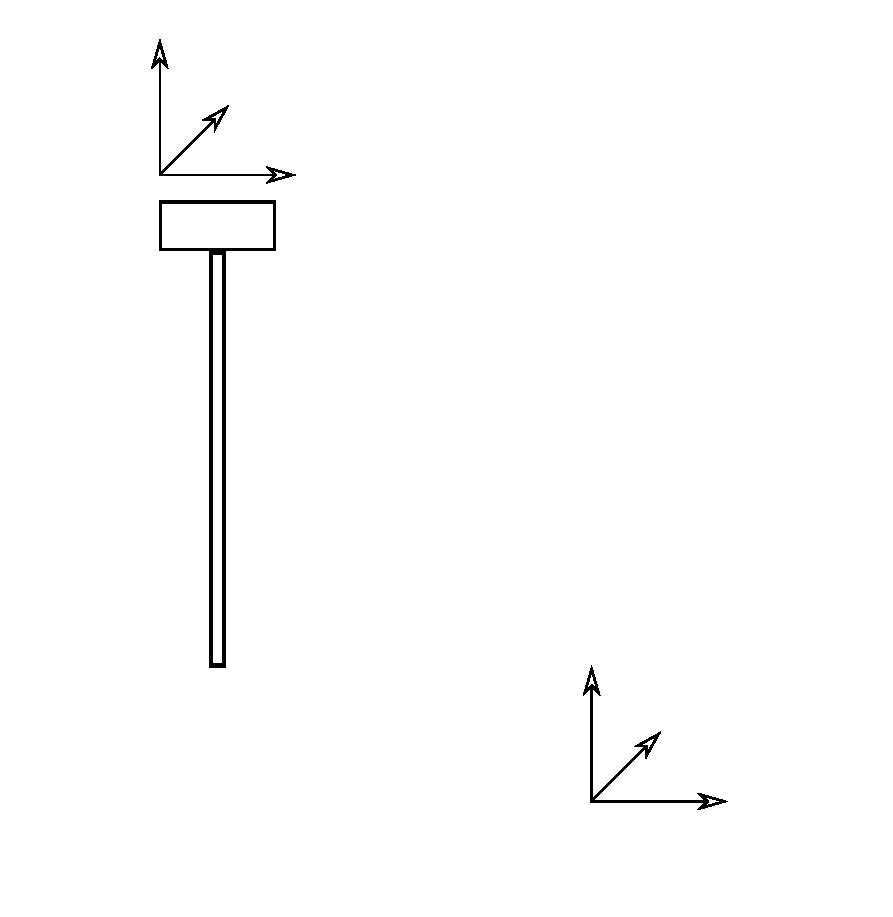
\includegraphics[width=0.8\textwidth]{figures/chapter5/test_flight_schem}
  %\def\svgwidth{200pt}
  %\input{figures/chapter5/test_flight_schem.pdf_tex}
  \caption[Shematic of the test flight layout.]{Schematic of the test flight, the quadcopter and CVS's respective axis systems and the offset vector between them.}
\label{fig:chap5-flight-test-schem}
\end{figure}

Furthermore, any angular offset for the CVS camera or the Suncopter due to uneven ground conditions or imperfect camera placement is also included in the offset vector. This makes the offset vector a six-dimensional position and orientation vector. The offset vector is a constant value and is related to the quadcopter and CVS's pose estimate by the relation given in Equation~\ref{eq:chap5-pose-offset}, where $\bm{P}$ is a six-dimensional pose vector. 

\begin{equation}
  \label{eq:chap5-pose-offset}
  \bm{P}_{\mathrm{quadcopter}} = \bm{P}_{\mathrm{CVS}} + \bm{P}_{\mathrm{offset}}
\end{equation}
Here, the $\bm{P}_{\mathrm{offset}}$ term is the unknown term. The pose data contained within the $\bm{P}_{\mathrm{quadcopter}}$ and $\bm{P}_{\mathrm{CVS}}$ terms contain noise in each sample, which requires an optimisation procedure be used to find a offset vector that best relates the two sets of pose data. For the optimisation procedure, the cost function and error term in Equation~\ref{eq:chap5-err-func} was minimised, where the error vector $\bm{e}$ is a function of $\bm{P}_{\mathrm{offset}}$ and $n$ is the number of samples in the data set. $\bm{e}$ is given by Equation~\ref{eq:chap5-err-term}. 

\begin{equation}
  \label{eq:chap5-err-func}
  \text{Cost function} = \min_{\bm{e}}\sqrt{\displaystyle\sum_{i=1}^{n} \bm{e}(\bm{P}_{\mathrm{offset}})_i^2}
\end{equation}

\begin{equation}
  \label{eq:chap5-err-term}
  \bm{e}_i = \bm{P}_{\mathrm{CVS}, i} + \bm{P}_{\mathrm{offset}, i} - \bm{P}_{\mathrm{quadcopter}, i}
\end{equation}
The minimisation was done using the \emph{minimize()} function from the SciPy\footnote{SciPy scientific tools library v0.13.3} library for the Python language, which makes use of the \emph{BFGS} quasi-Newton method described by~\cite{nocedal2006numerical}. 

\subsubsection{Determining the Pose Estimation Error}

With the two data sets now directly relatable, the pose estimation error of a quadcopter in flight can now be determined by using the RBFNN discussed in Chapter~\ref{chap4} and the two sets of pose data recorded during the flight tests.  

The input to the network is the CVS's recorded pose data. The network then outputs the expected measurement error for every sample, allowing a measurement error band to be drawn around the CVS's measurement data. This error band can then be used to determine if the quadcopter or the CVS's pose estimates are more accurate: when the quadcopter's estimate falls within the error band, it indicates that the quadcopter's pose estimate is more accurate for that sample than the CVS's estimate is, while the opposite holds true if it falls outside the error band. It can then be determined which of the two systems produce on average the most accurate pose measurements. However, if it is found that the quadcopter's pose estimate is more accurate, one might be liable to ask if the CVS is still necessary.

Up to this point, any measure of a quadcopter's pose estimation error has been unavailable for outdoor quadcopters. This means that even if it is found that the quadcopter's pose estimate is more accurate than the CVS's, the CVS pose data will still provide a worst-case measure of the quadcopter's pose estimate which was not available previously. 

The outcome of this comparison may lead to one of the following two outcomes: if the quadcopter's pose estimate is more accurate than the CVS's, the pose measurement error of the CVS can be taken as a quadcopter's worst-case pose measurement error, where the quadcopter's pose estimate will always be at least as accurate as, but likely better than the CVS's. Conversely, if it is found that the CVS produces better pose measures, then the quadcopter's pose estimation error will be given by the difference between the CVS and quadcopter's pose data. 

\section{Results}

The results for the offset vector, $\bm{P}_{\mathrm{offset}}$, and the pose estimation error is presented and discussed in this section. 

\subsection{Offset Vector}

Using the procedure described in Section~\ref{sec:chap5-data-centring}, the optimal offset vector relating the quadcopter and CVS's axis systems is given by 

\begin{equation}
  \label{eq:chap5-offset-result}
  \bm{P}_{\mathrm{offset}} = 
  \begin{bmatrix}
    \SI{-6.61}{\m} & \SI{-0.834}{\m} & \SI{-4.17}{\m} & \ang{6.15} & \ang{62.7} & \ang{-185} \\
  \end{bmatrix}^T.
\end{equation}
The position values roughly coincide with the conditions that were recorded on site: the Suncopter was launched some distance from the CVS equipment for safety reasons. Furthermore, due to uneven ground conditions at the testing site, the launch site was also slanted and located below the post on which the CVS's camera was placed. Thus, from a sanity check point of view, the offset that the optimisation procedure produced seems to be the correct one. 

\subsection{Pose Estimation Error}

Several different flight tests were conducted with different flight conditions. However, for convenience, only the results from the $\SI{1}{\m}$ altitude and $\ang{0}$ yaw case are presented and discussed. There is nothing special about this case and the data results from all the flight tests produce roughly the same results.  

Before the flight test data was fed to the RBFNN, it was first checked that the test data fell within the training data limits. This is done to ensure that the RBFNN is not exposed to data it was not trained for and produce inaccurate results. Figure~\ref{fig:chap5-ts-tr-scatter} shows scatter plots for the test and training data dimensions and shows that the test data falls comfortably within the training data set limits.  

\begin{figure*}
  \centering
  \begin{subfigure}{\textwidth}
    \begin{subfigure}{0.48\textwidth}
      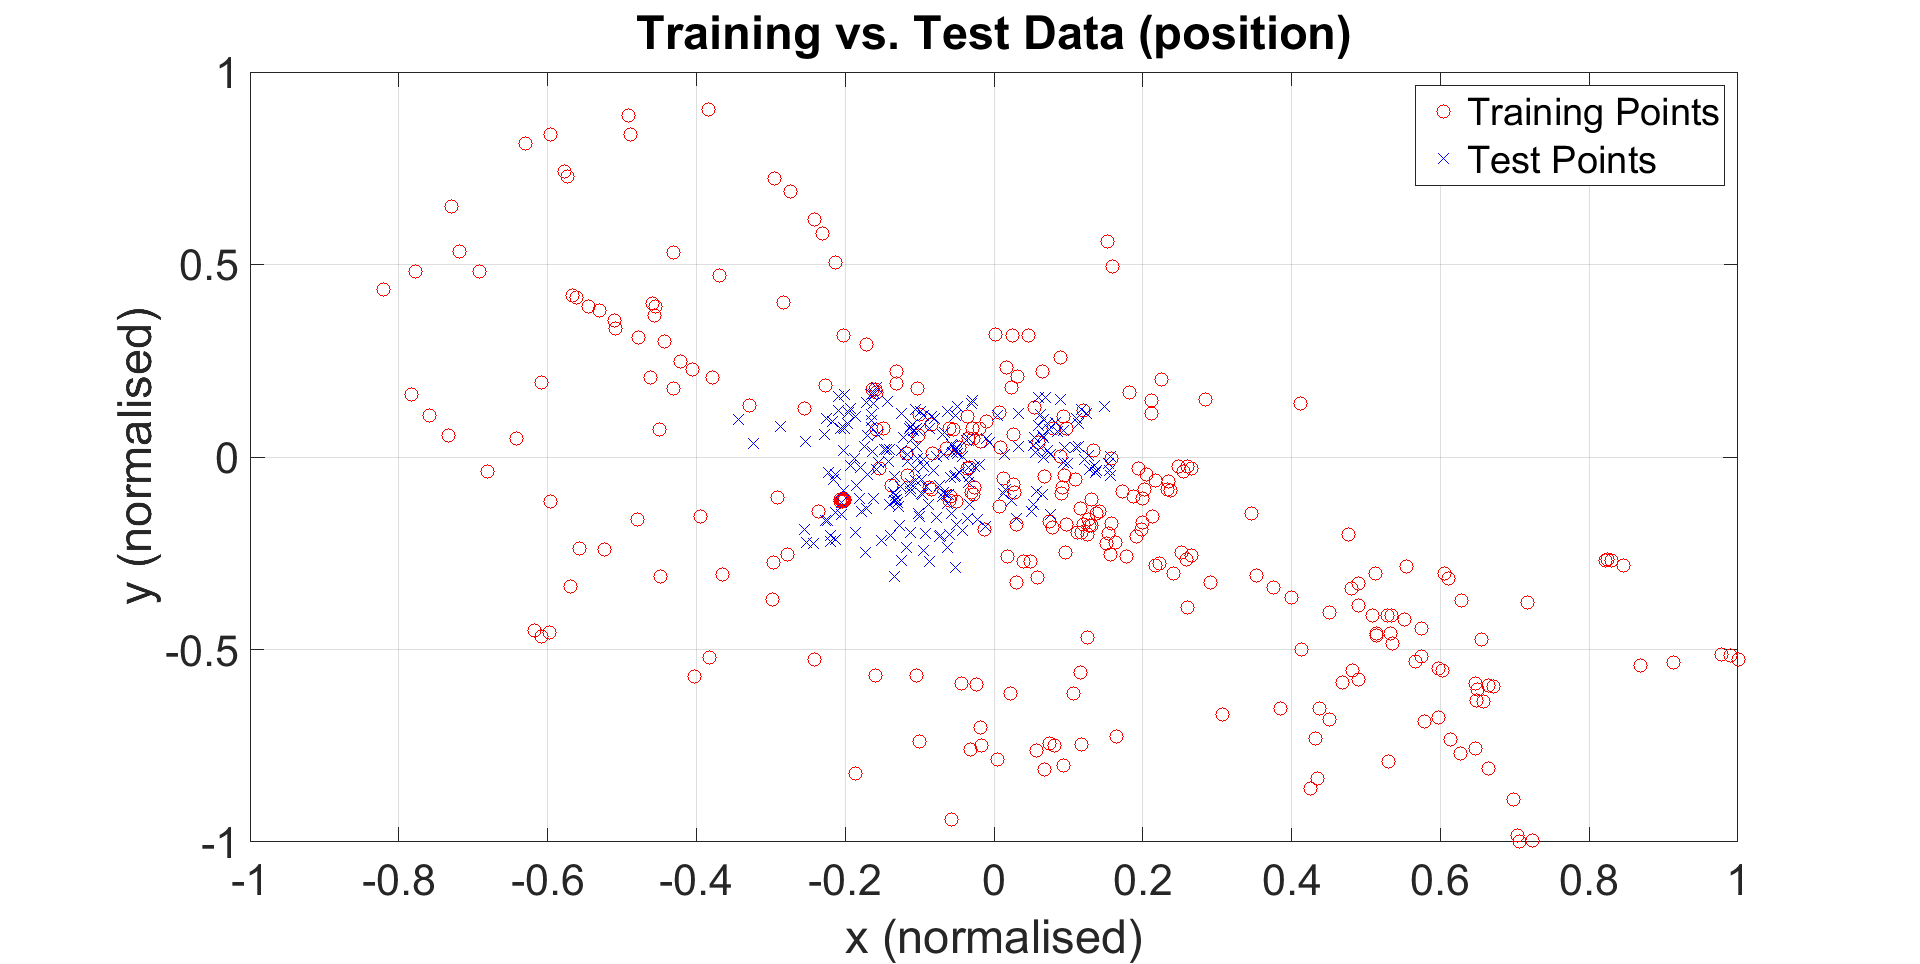
\includegraphics[clip, trim = 80 0 80 0, width=\textwidth]{figures/chapter5/trts_xy}
    \end{subfigure}
    \begin{subfigure}{0.48\textwidth}
      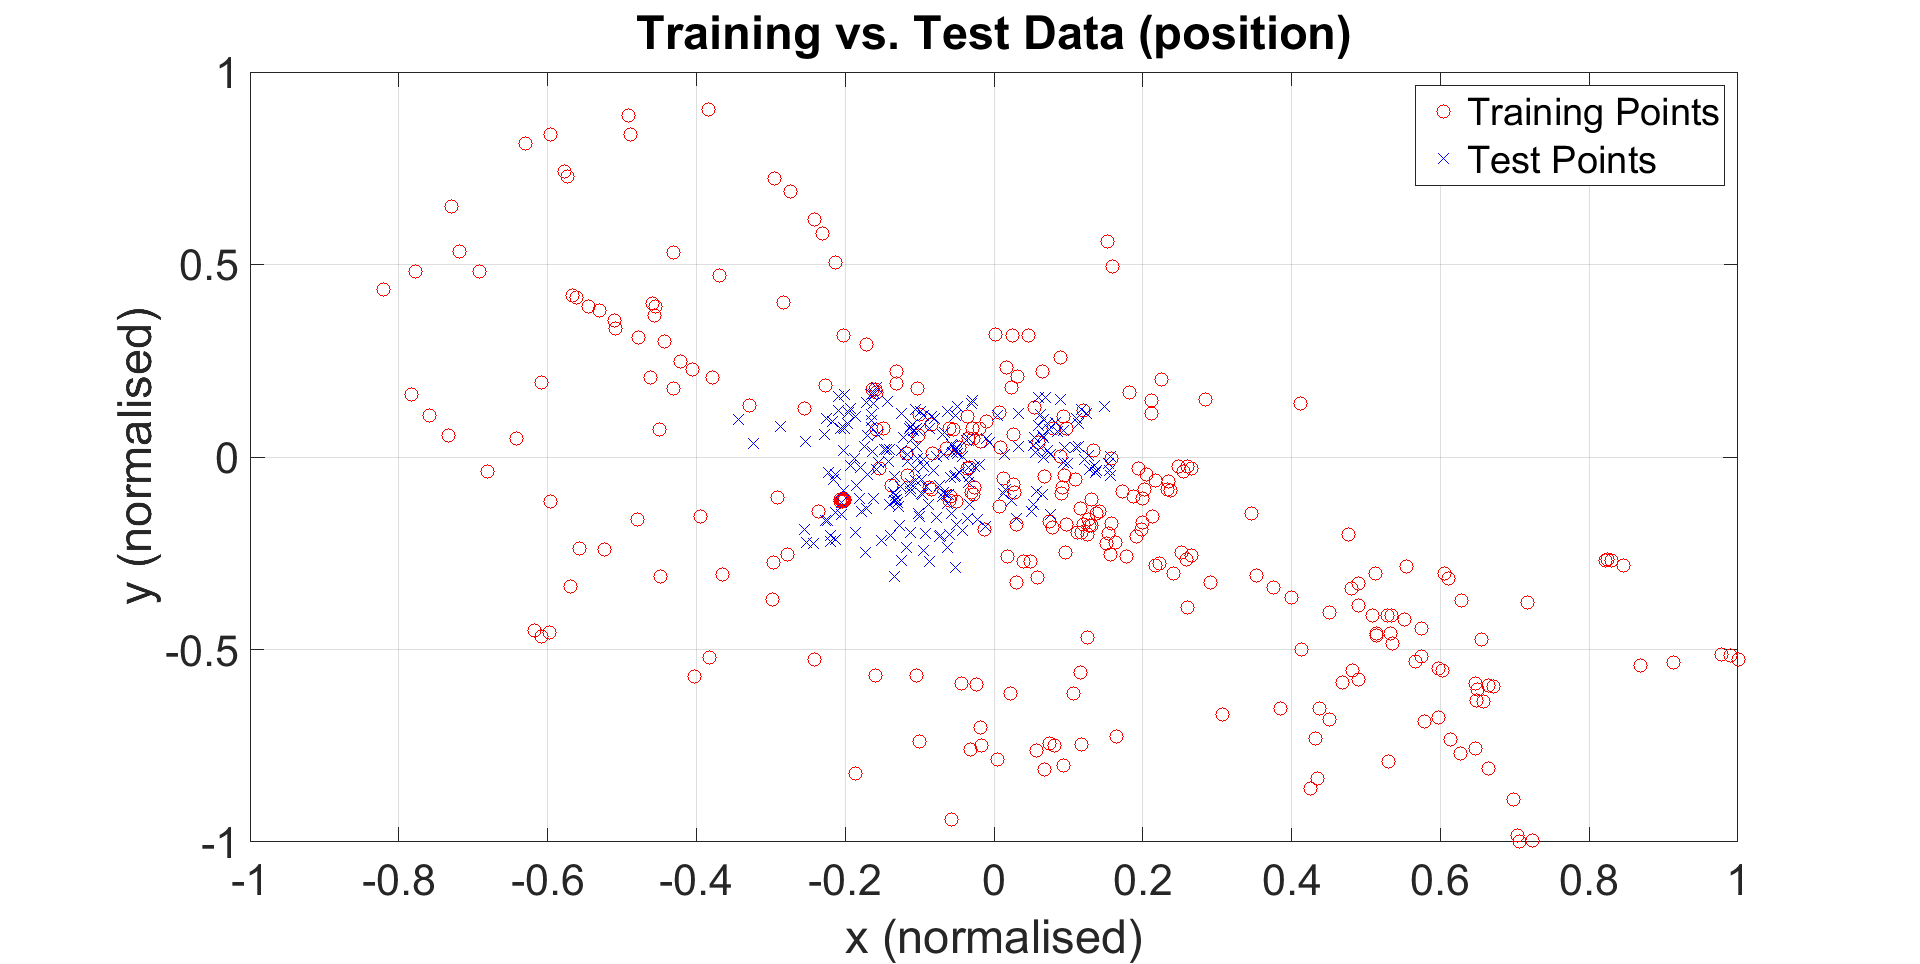
\includegraphics[clip, trim = 80 0 80 0, width=\textwidth]{figures/chapter5/trts_xy}
    \end{subfigure}
    \caption{}
  \end{subfigure}
  \begin{subfigure}{\textwidth}
    \begin{subfigure}{0.48\textwidth}
      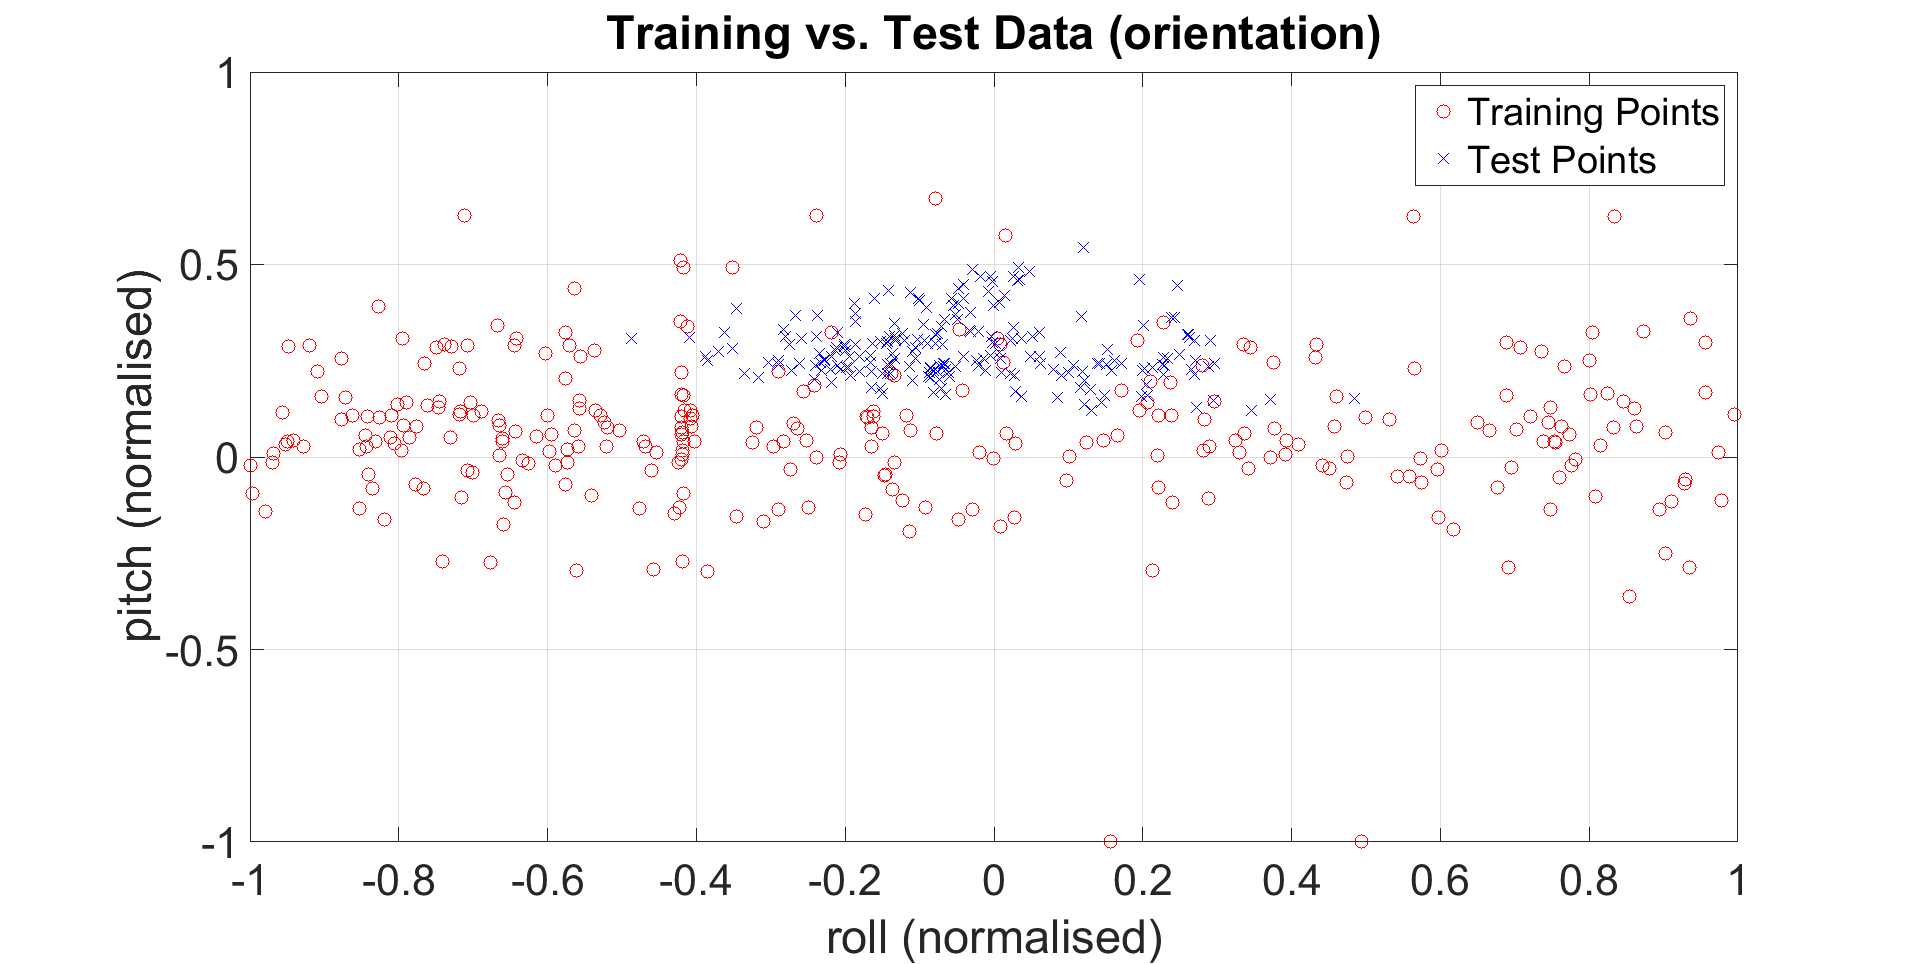
\includegraphics[clip, trim = 100 0 100 0, width=\textwidth]{figures/chapter5/trts_rollpitch}
    \end{subfigure}
    \begin{subfigure}{0.48\textwidth}
      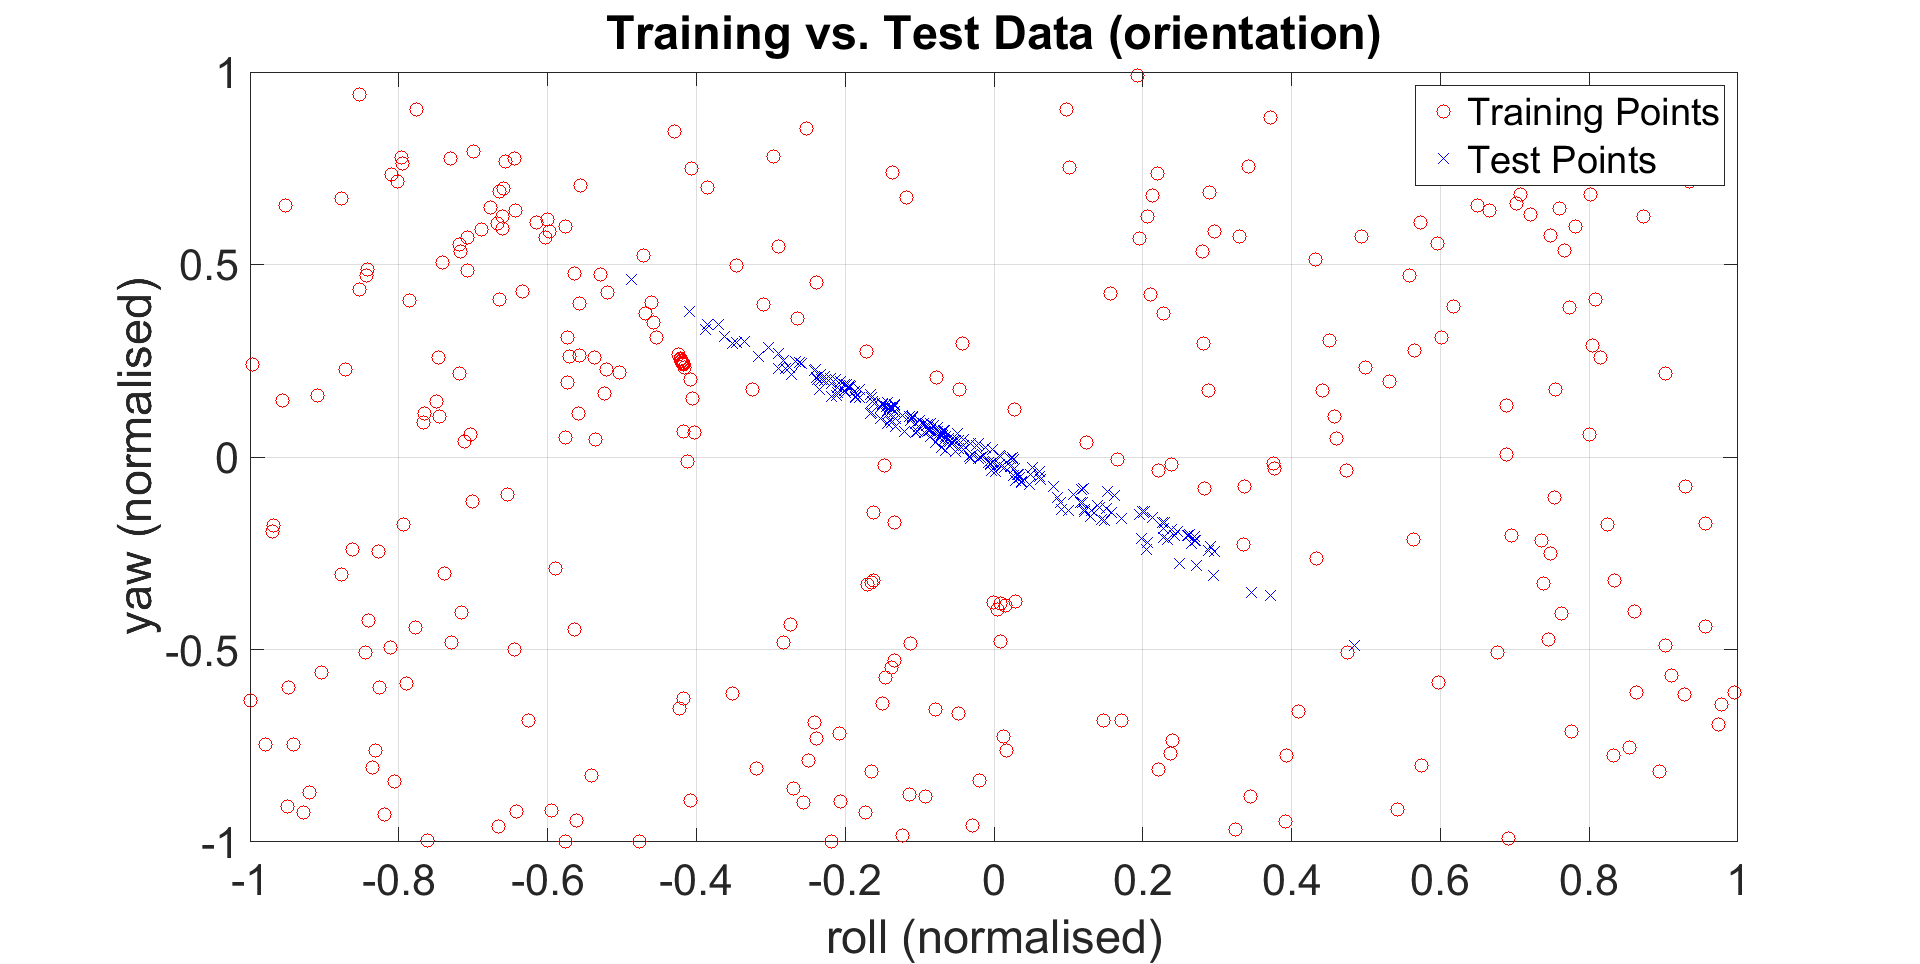
\includegraphics[clip, trim = 100 0 100 0, width=\textwidth]{figures/chapter5/trts_rollyaw}
    \end{subfigure}
    \caption{}
  \end{subfigure}
  \caption[Scatter plots of flight data vs.\ training data. ]{Scatter plots showing that the flight test data falls within the training limits. }
\label{fig:chap5-ts-tr-scatter}
\end{figure*}

The results for the flight test are presented in Figure~\ref{fig:chap5-results}. Here, six figures are given which plot the different pose dimensions. Each plot contains the Suncopter's pose estimate, as well as the expected measurement error margin for the CVS as given by the RBFNN.\@ It can be observed from the plots for the $z$ and $yaw$ dimensions that they consistently hover around the flight configuration's set point of $\SI{1}{\m}$ and $\ang{0}$, providing a degree of sanity to the measurements. 
  
\begin{figure*}
  \centering
  \begin{subfigure}{0.48\textwidth}
    \begin{subfigure}{\textwidth}
      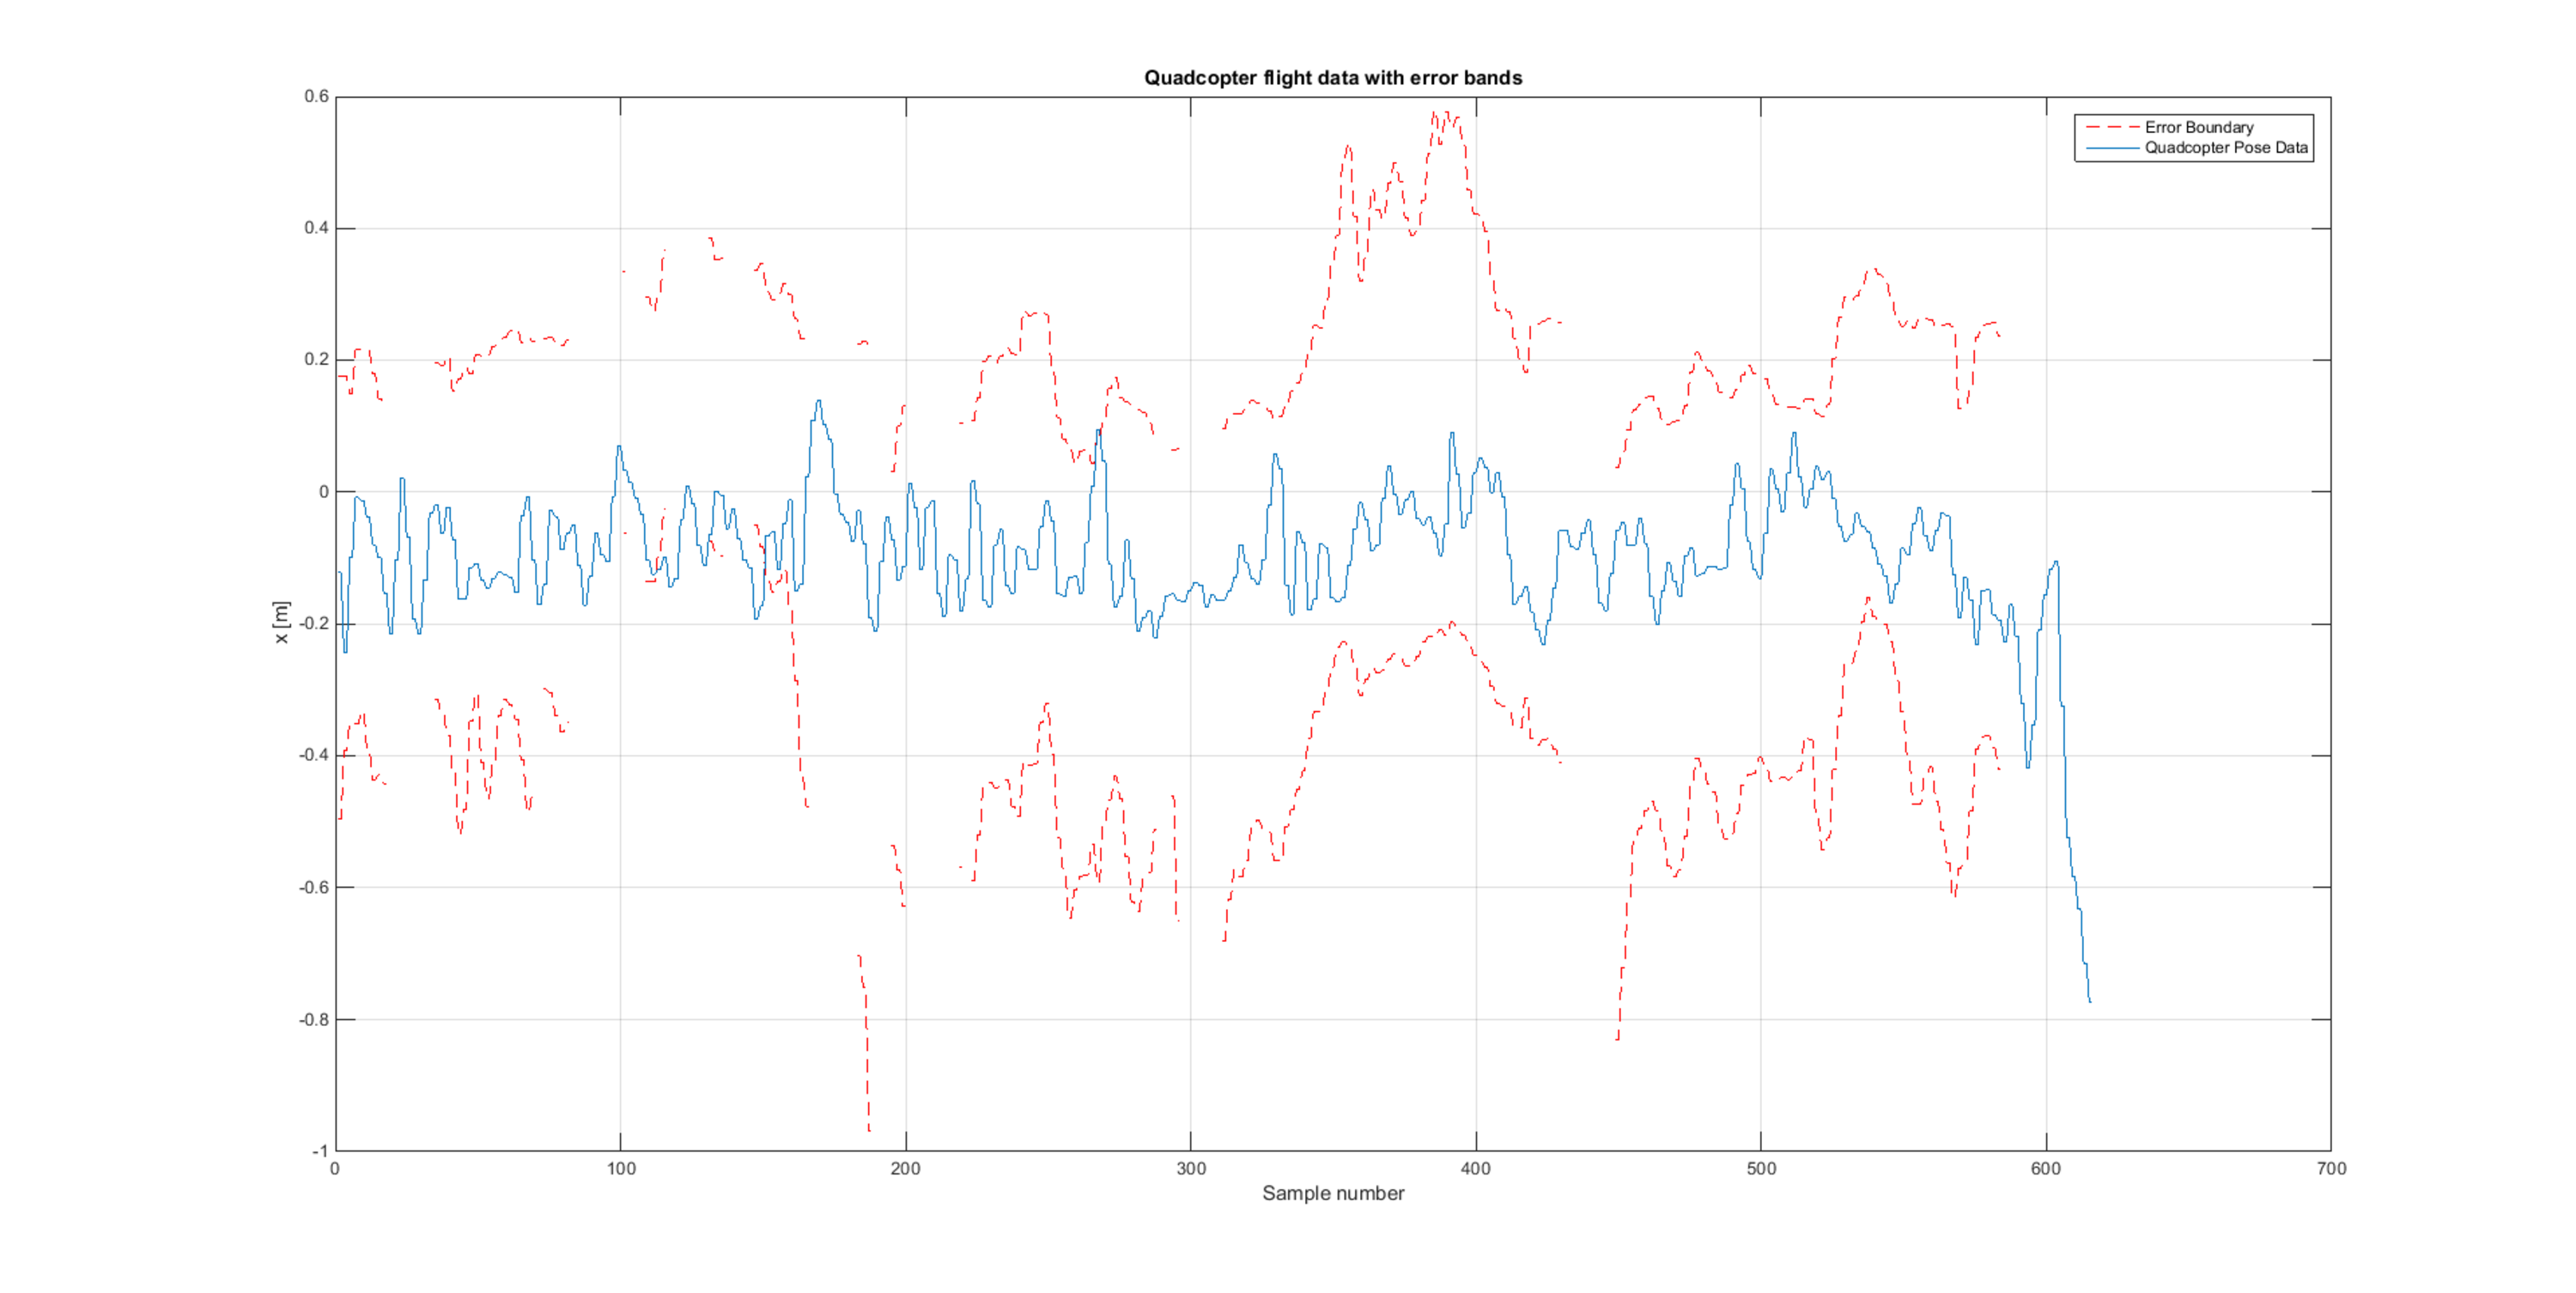
\includegraphics[clip, trim = 100 0 100 0, width = \textwidth]{figures/chapter5/x}
    \end{subfigure}
    \begin{subfigure}{\textwidth}
      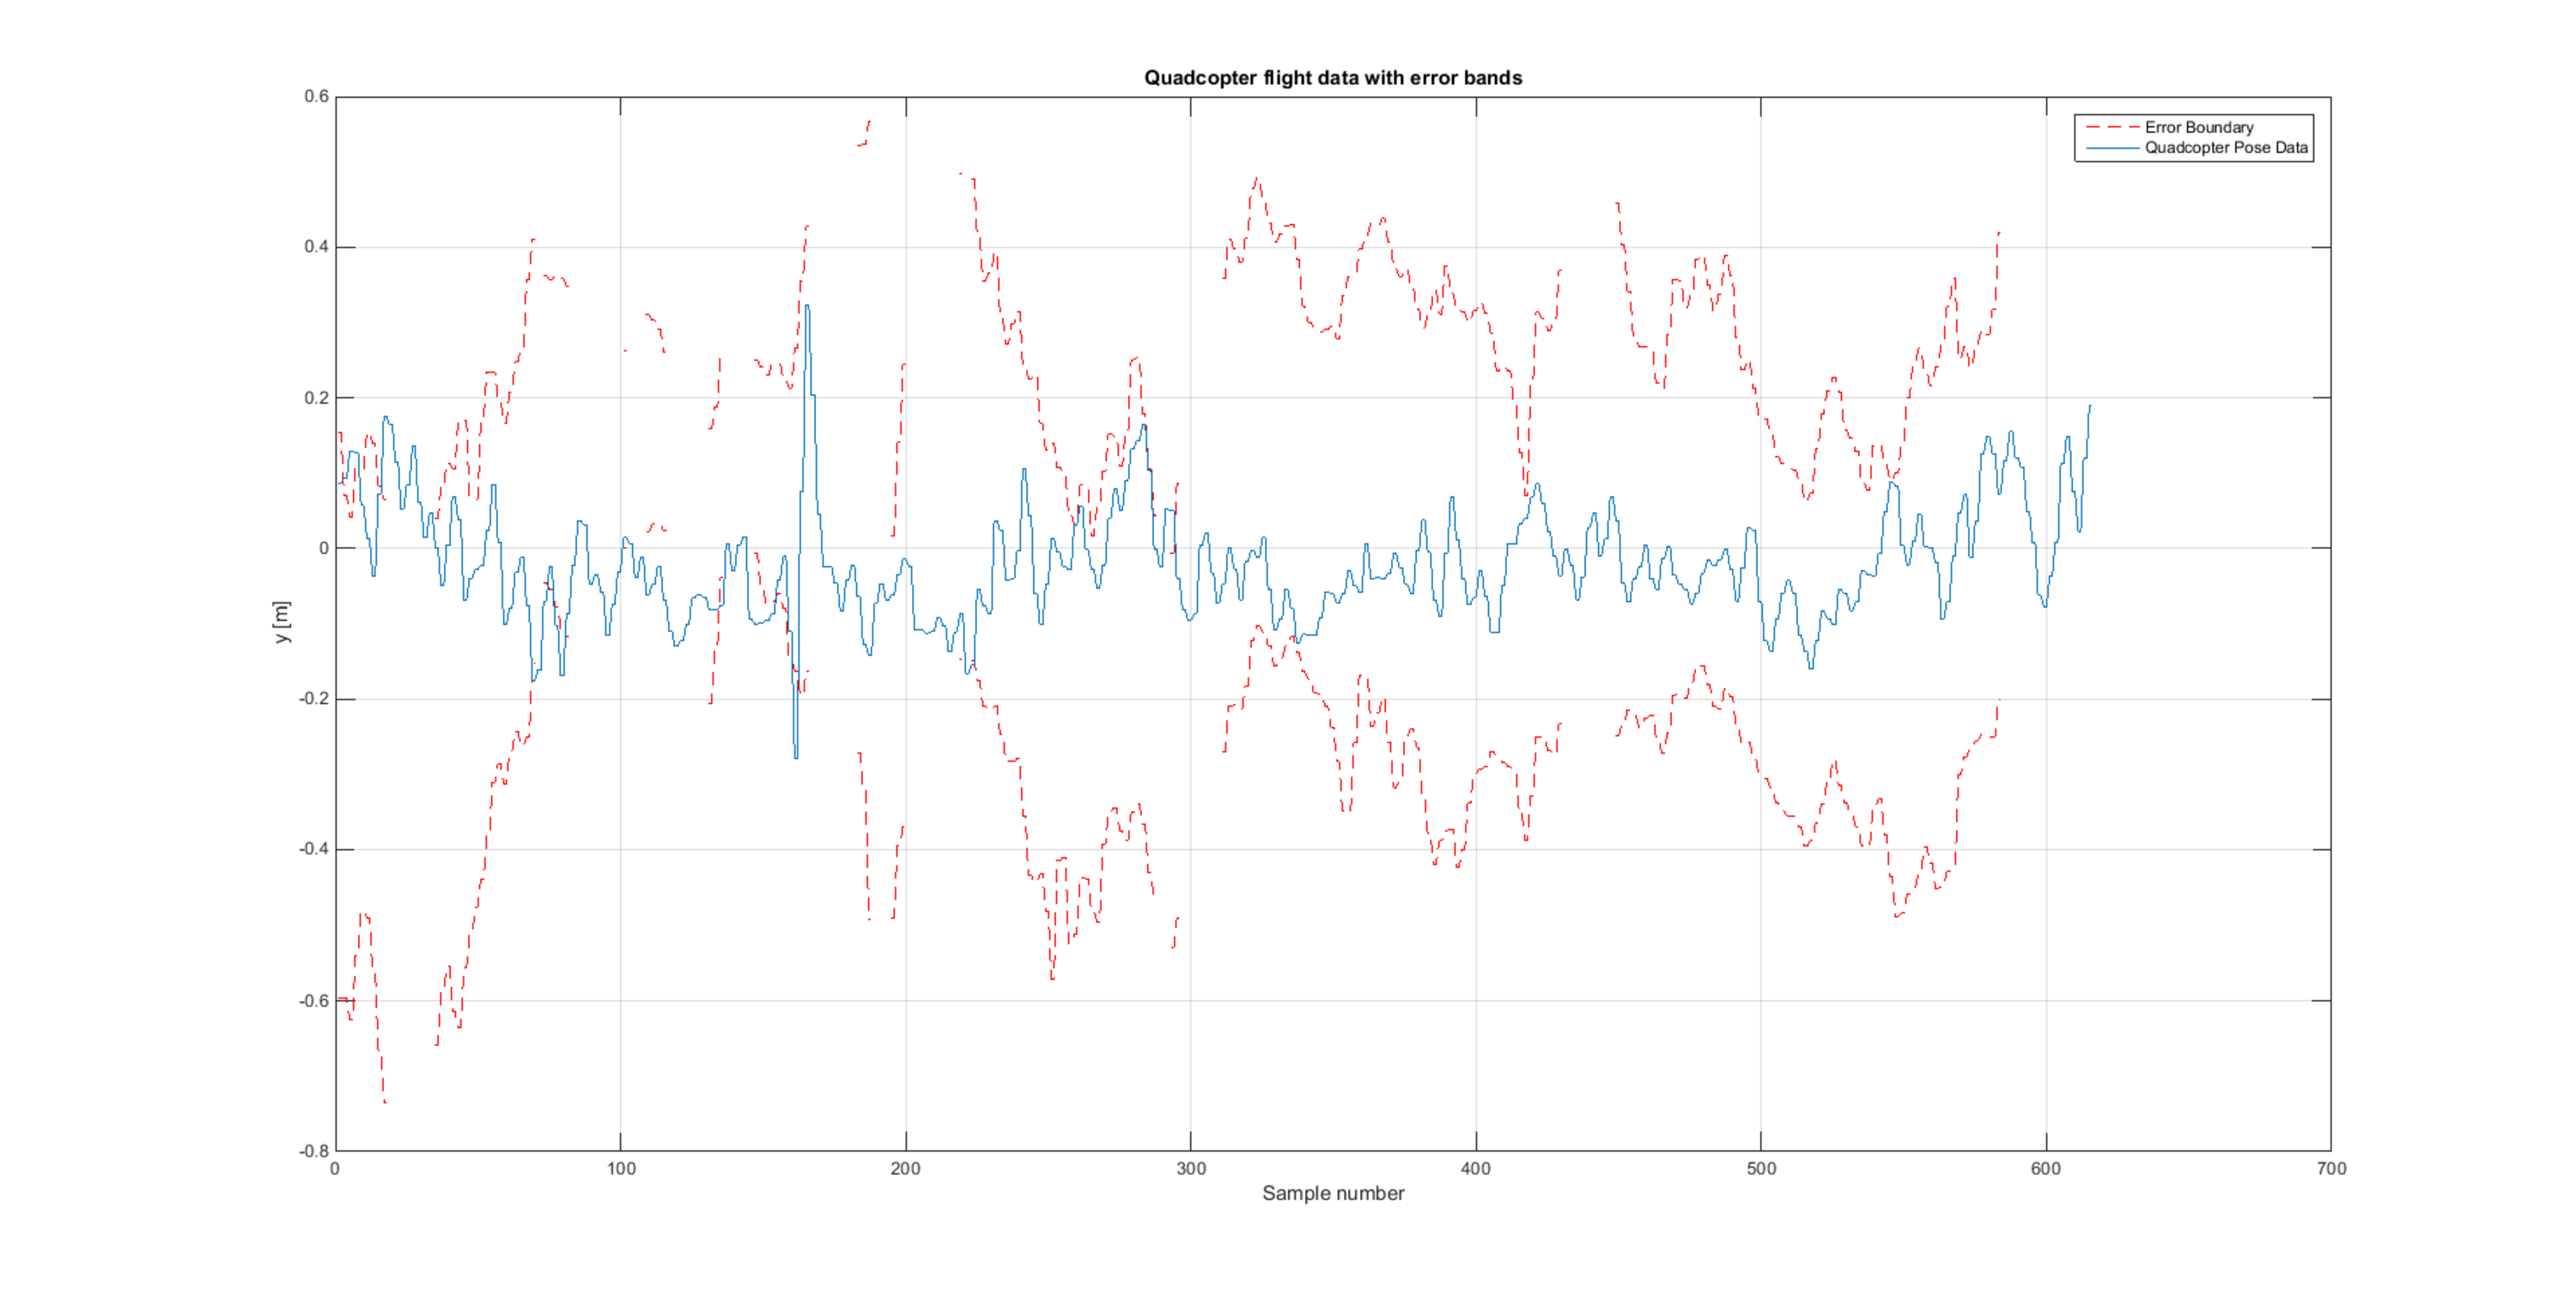
\includegraphics[clip, trim = 100 0 100 0, width = \textwidth]{figures/chapter5/y}
    \end{subfigure}
    \begin{subfigure}{\textwidth}
      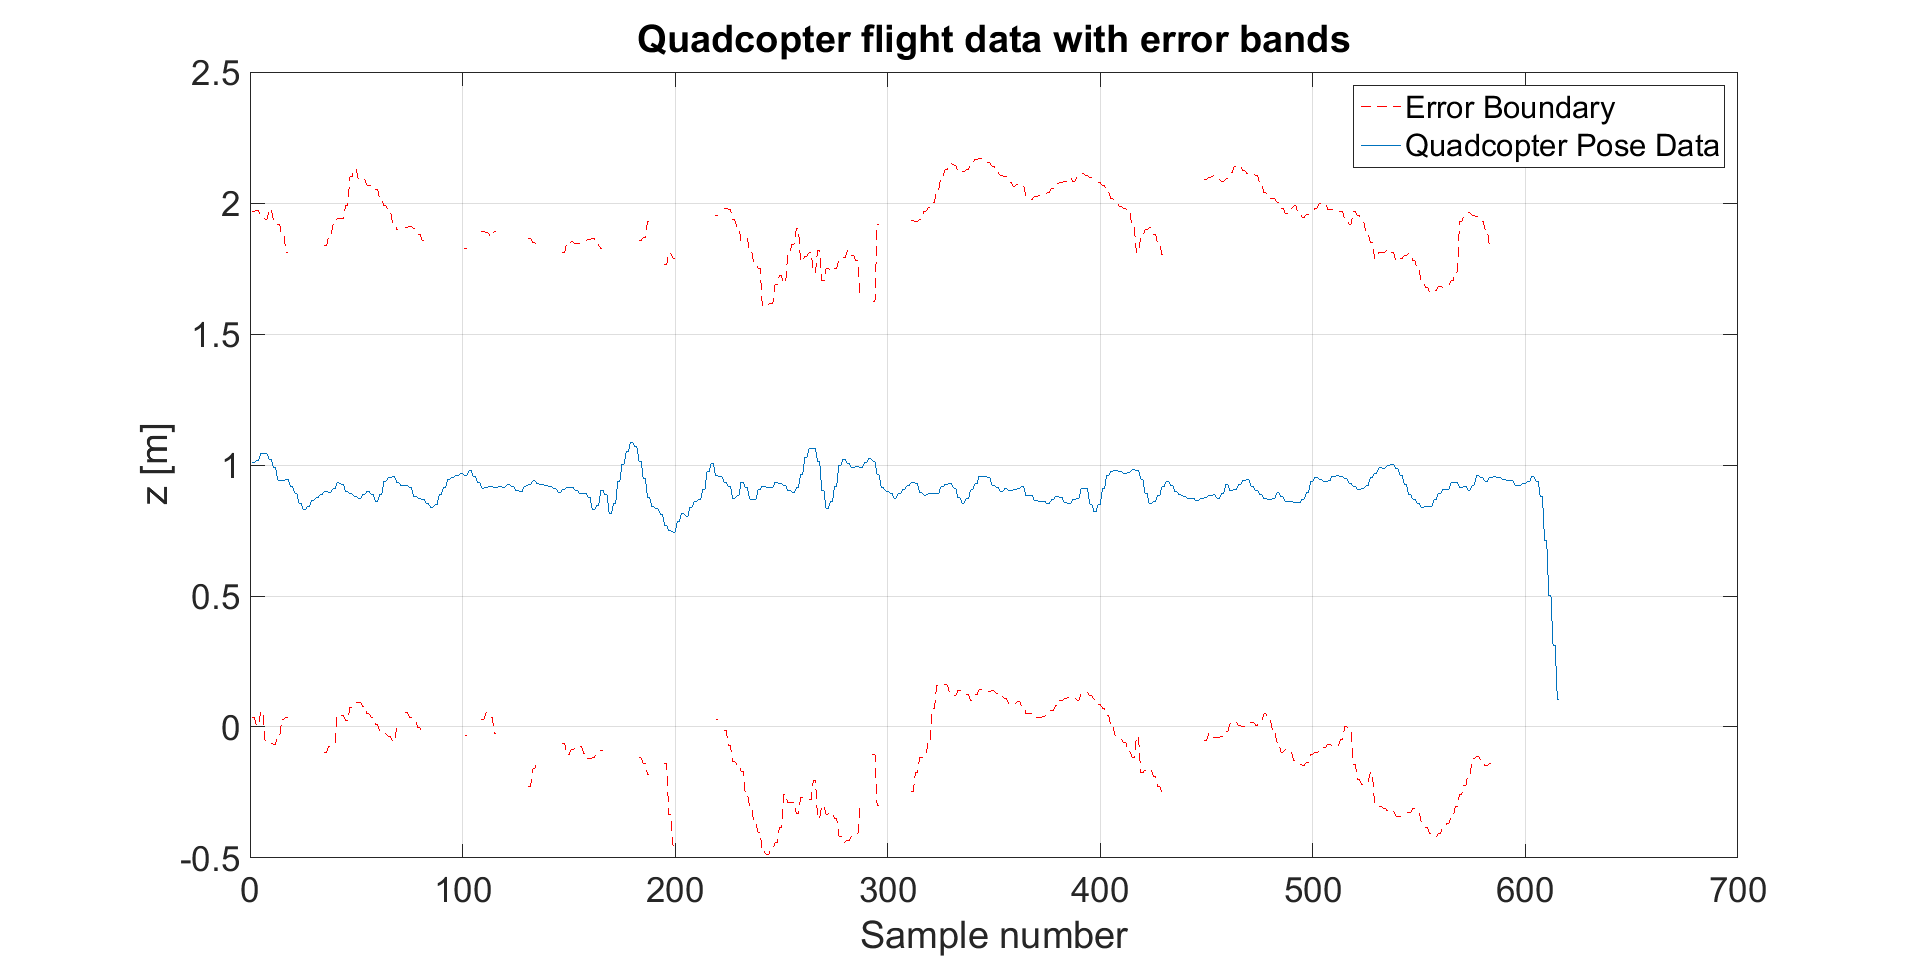
\includegraphics[clip, trim = 100 0 100 0, width = \textwidth]{figures/chapter5/z}
    \end{subfigure}
    \caption{}
  \end{subfigure}
  \begin{subfigure}{0.48\textwidth}
    \begin{subfigure}{\textwidth}
      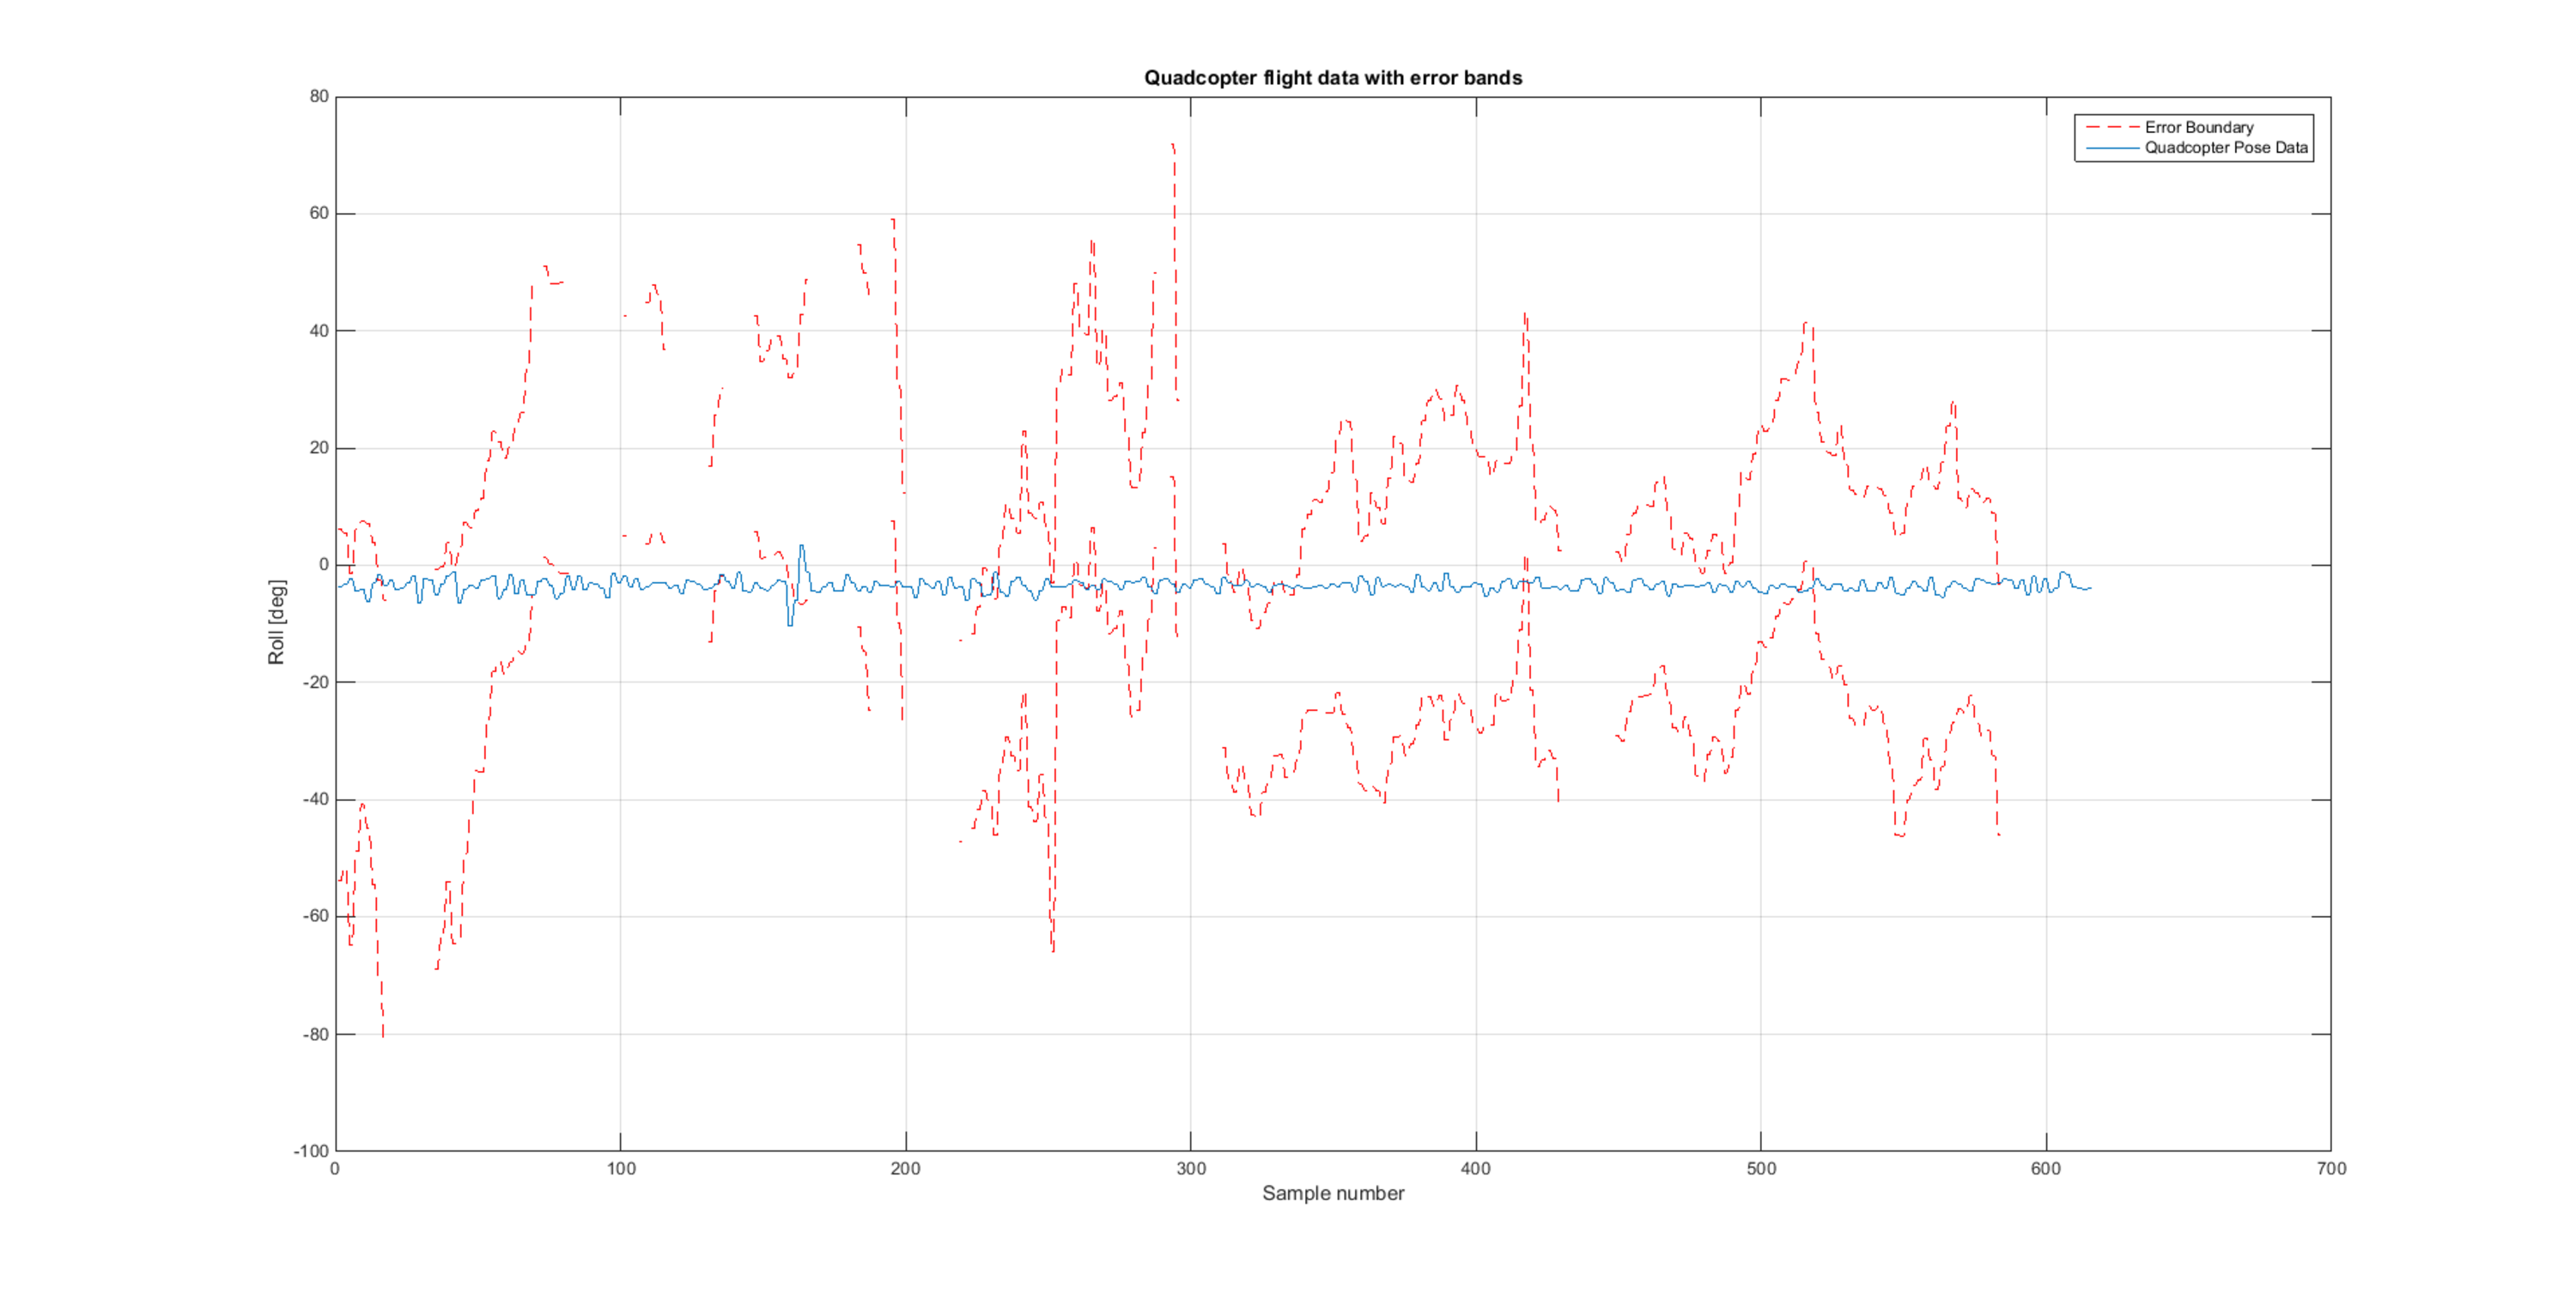
\includegraphics[clip, trim = 100 0 100 0, width = \textwidth]{figures/chapter5/roll}
    \end{subfigure}
    \begin{subfigure}{\textwidth}
      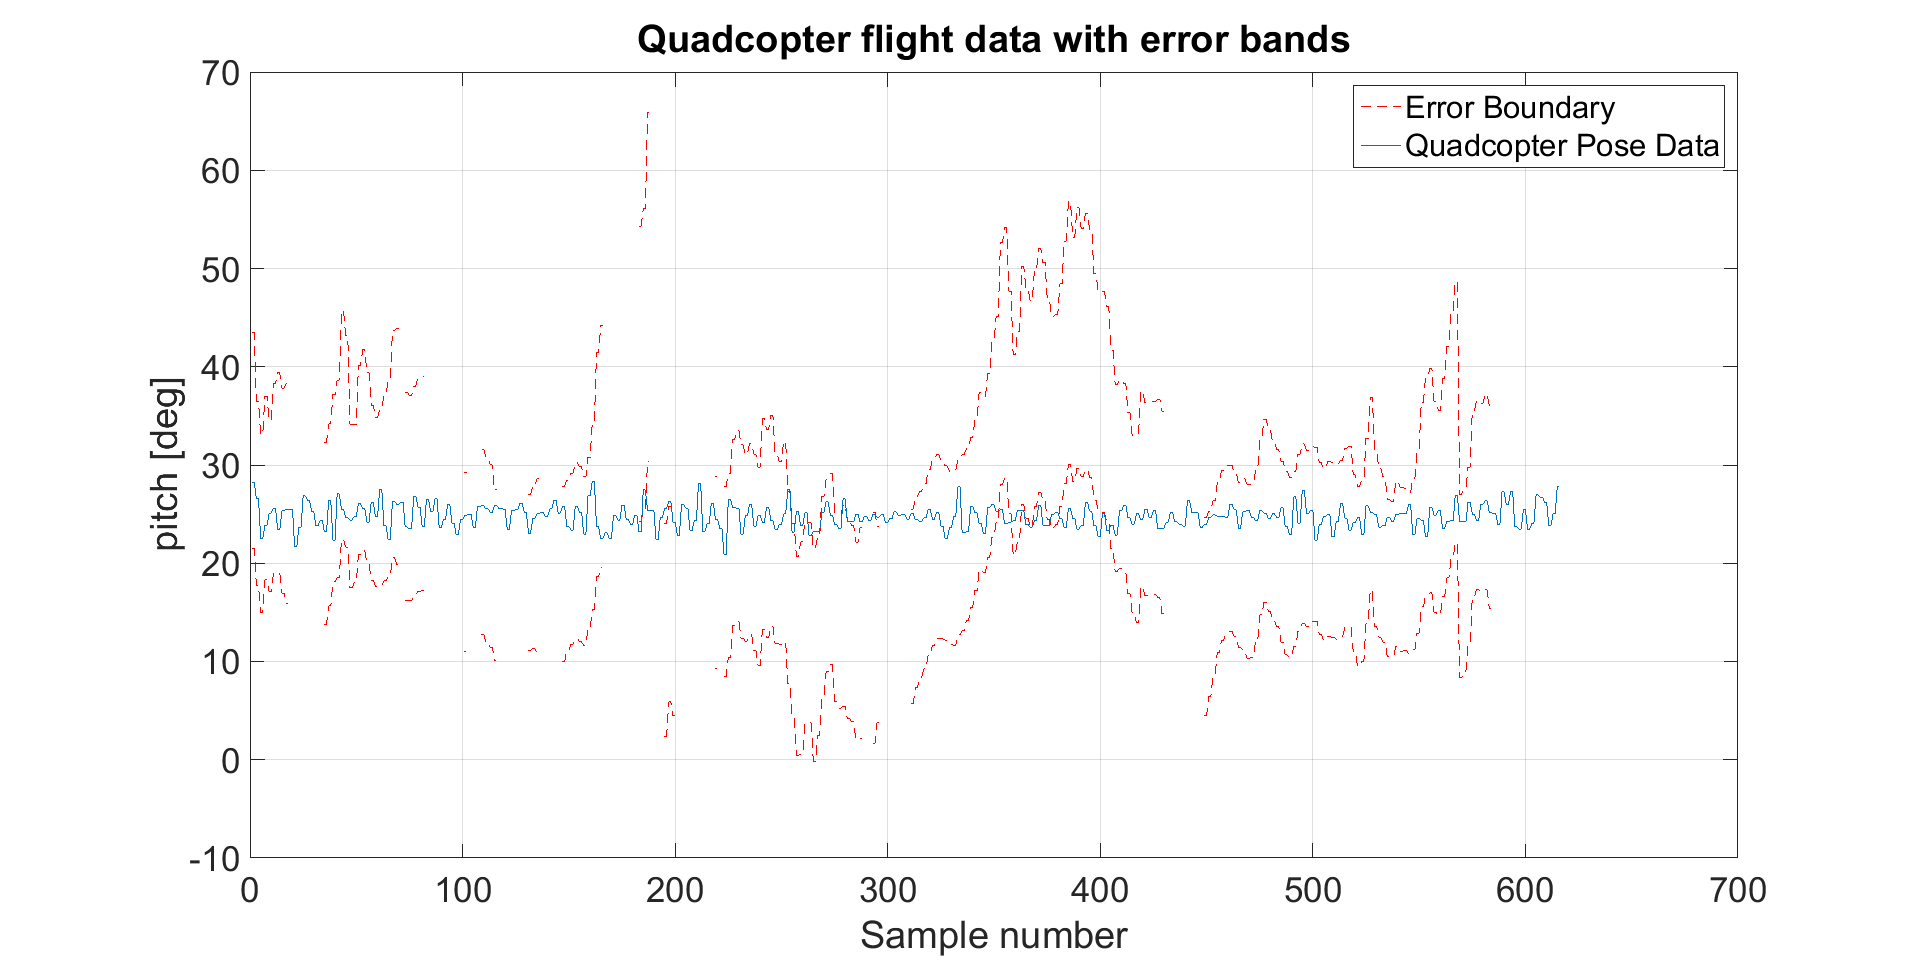
\includegraphics[clip, trim = 100 0 100 0, width = \textwidth]{figures/chapter5/pitch}
    \end{subfigure}
    \begin{subfigure}{\textwidth}
      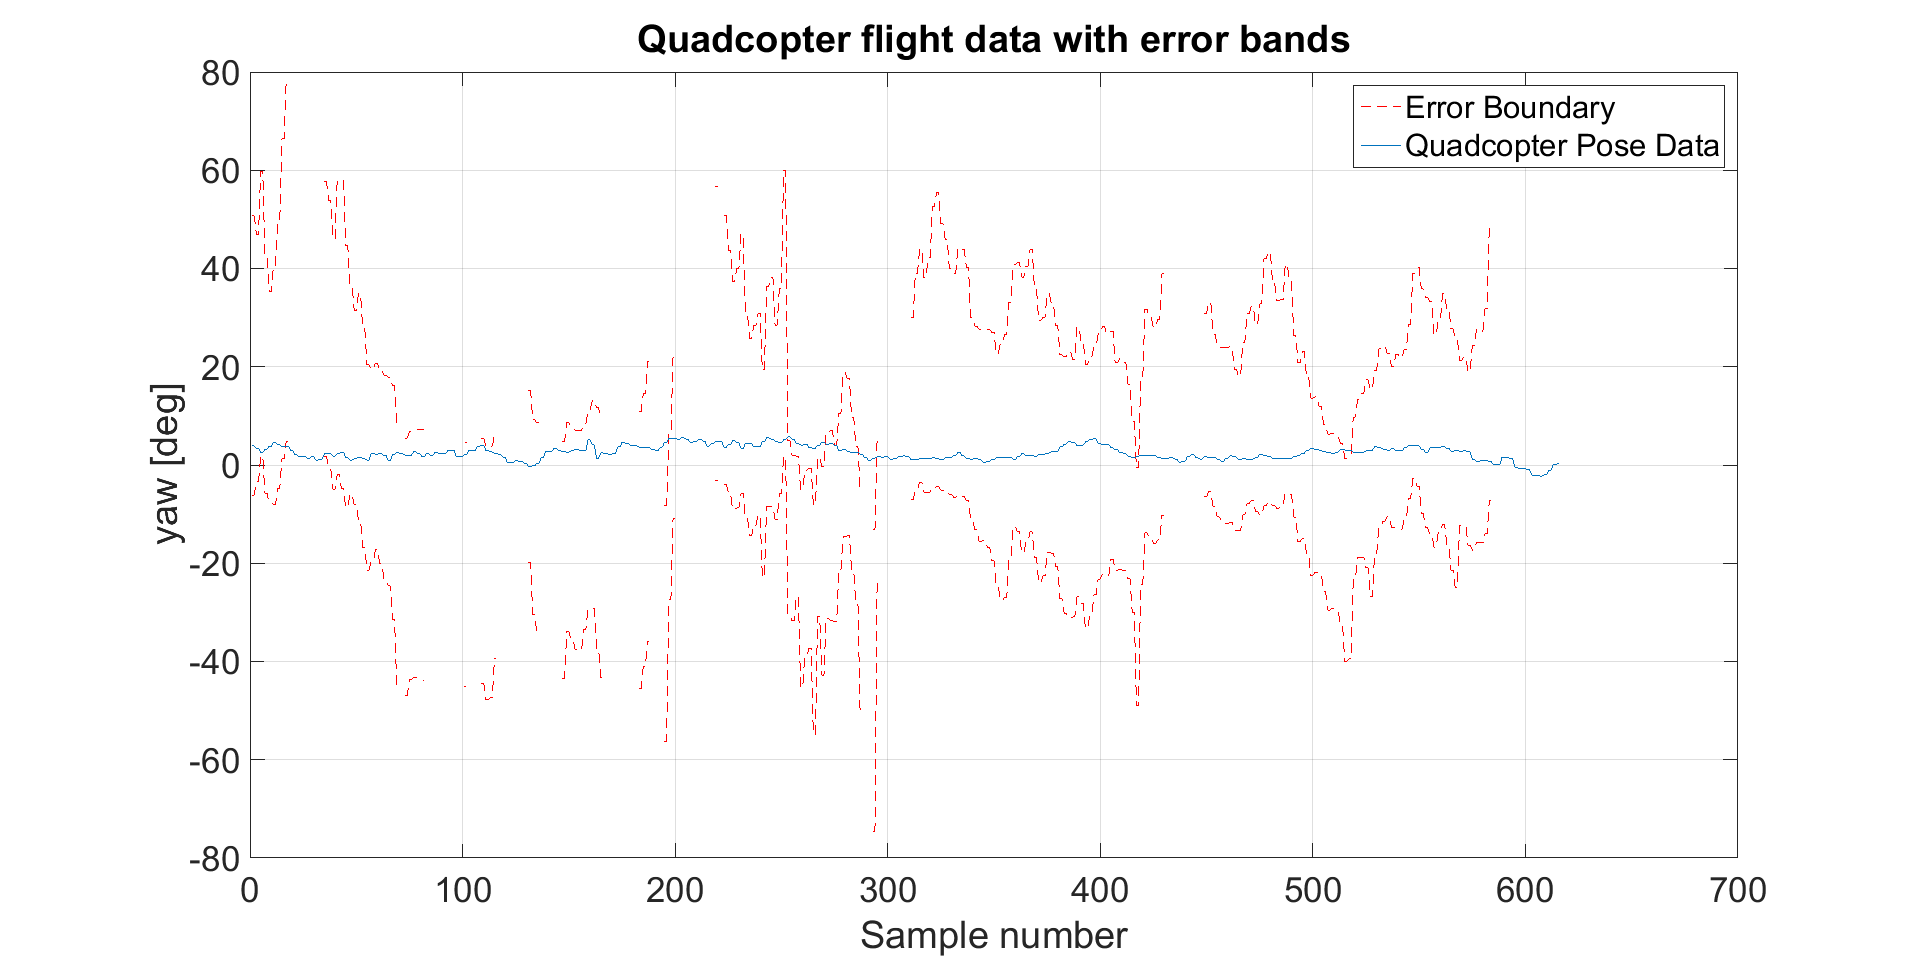
\includegraphics[clip, trim = 100 0 100 0, width = \textwidth]{figures/chapter5/yaw}
    \end{subfigure}
    \caption{}
  \end{subfigure}
\caption[Plots of the Suncopter's flight and measurement errors.]{Plots of the Suncopter's pose estimate with the error margins from of the CVS's pose measurement. }
\label{fig:chap5-results}
\end{figure*}

The first important aspect to note of the plots in Figure~\ref{fig:chap5-results} is that the quadcopter's estimate largely falls within the error boundaries for the CVS's pose measurement. This implies that the pose estimate given by the quadcopter's sensor suite is more accurate than the CVS's measurements, especially with its orientation estimate where the CVS has a large area of uncertainty. The RBFNN has been adequately trained in Chapter~\ref{chap4} and Figure~\ref{fig:chap5-ts-tr-scatter} shows that the test data falls within the training data limits, giving a degree of certainty that the quadcopter's true position falls within the extreme CVS pose measurement errors. It therefore follows that the measurement error of the CVS can be taken as a worst-case pose estimation error for the Suncopter. 

Secondly, there are sections in the CVS error estimate plots which are missing. The reason for this is that during the video recording, the calibration board went out of the CVS camera's field of view or it could not detect enough of the corners due to bad lighting conditions or the board being to far from the camera. These effects were somewhat remedied by adjusting the pose extractor to use an adaptive threshold filter on the video data and can be permanently fixed by flying the quadcopter closer to the camera or ensuring that the board is well and evenly lit. 

\section{Conclusion}

In this chapter, the CVS and RBFNN was used to measure the pose of an airborne quadcopter in the outdoors and to find the quadcopter's pose estimation accuracy. It was found that the quadcopter's on-board pose estimate is more accurate than the CVS's.\@ However, the CVS's pose measurement error can still be used to provide a measure of how accurately the quadcopter can estimate its position, since its estimates will, at worst, be as accurate as the CVS's.\@ 
